% !TEX encoding = UTF-8 Unicode
\documentclass[10pt, a4paper]{article}

%% Page Margins
\usepackage[top=1in,right=1in,bottom=1in,left=1in]{geometry}

\title{UnBabel - Data Science Challenge}
\author{Rion Brattig Correia}
\date{}

%% References
\usepackage{natbib}

%% Images
\usepackage{graphicx}

%% Colors
\usepackage{xcolor}
\definecolor{linkcolor}{rgb}{0,0.2,0.6}

%% HyperLinks on References
\usepackage{hyperref}
\hypersetup{
    colorlinks=true,
    breaklinks=true,
    citecolor=linkcolor,
    linkcolor=linkcolor,
    filecolor=magenta,      
    urlcolor=linkcolor,
}

%% Clever Ref
\usepackage{cleveref}


\begin{document}

\maketitle


\section{Executive Summary}


\textbf{Client complains} on unstable quality of translations can be solved by assigning editors to tasks from topics they have a minimum level of proficiency (e.g., quality $\geq$ 3), rather than simply at random.
%
This will not impact the pool of editors, since 93.78\% of editors have at least a translation quality of 3 in at least one particular topic.
%
That is to say editors who are very good in one particular topic often lack skills in another, and vice versa (see \cref{fig:tranferable-skills}). Similar results are found in other domains.
%
Only three (3) editors have a maximum translation quality of 2 or less in any particular topic. Since these represents a small percentage of editors (0.72\%), we recommend getting in touch with these editors to discuss possible ways to improve their translation quality in the topic they are most proficient.
%
However, this result may not represent the full picture of the problem, which is related to editor language pairs, as we describe below.


\textbf{Complains from editors} who are not getting any task is troublesome. If tasks as indeed randomly assigned (e.g., uniform distribution), all editors have an equal chance of receiving a task.
%
We suspect these complains could be associated with a majority of editors having few particular language pairs (e.g., most editors are \texttt{pt\_en} only). Since the distribution of task is associated with a matching of language pairs between task and editor, a large imbalance in language pair supply versus demand could be driving the observed phenomena.
%
However, our current dataset does not allow us to answer this question properly as we are unable to link language pairs between tasks and editors.
%
The dataset will require to be updated for this suspicion to be ruled out entirely.



\section{Technical description and suggestions}


\begin{figure}[h!]
    \centering
    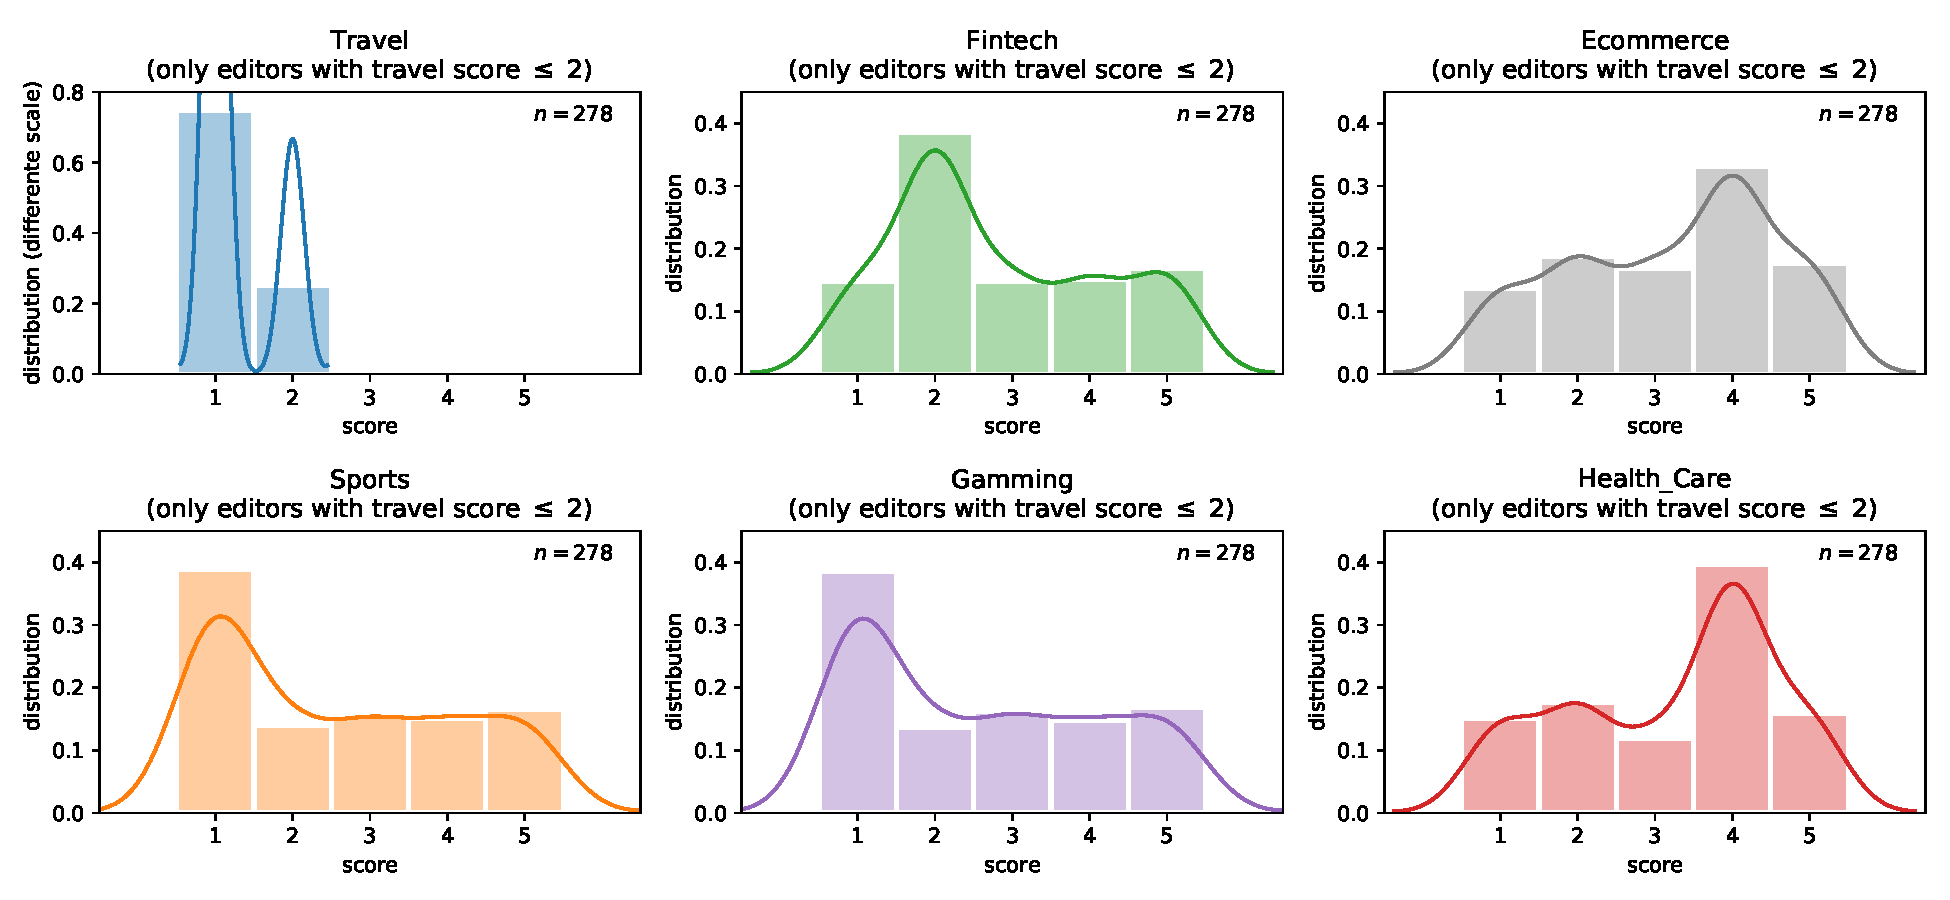
\includegraphics[width=\textwidth]{images/transferable-skills}
    \caption{
        Distribution of editors with low \texttt{travel} skills ($S_e(d_t) \leq 2$), across all other domains.
        %
        Note these same editors have higher skills in \texttt{ecommerce} and \texttt{health\_care} domains.
        %
        The upper left plot has a different scale.
    }
    \label{fig:tranferable-skills}
\end{figure}


There are several inconsistencies between the challenge instructions and the dataset that makes it difficult for a clear assessment of the problem in question---possibly on purpose.
%
For instance, the quality of a task, $Q(t)$, is based on a matching between the language pair of the task ($LP_{t}$) and the set of language pairs of the editor ($LP_{e}$). However the dataset does not specify the set of language pairs for each editor.
%
Also, the \textit{tickets} table contains a duplicated column name, \texttt{client\_id}. Values between these columns are different, but the relation of one of the duplicated column is not possible to be inferred from the data.
%
We would recommend the dataset to include the missing columns and fix column names.


Also, variable $P$ is used in two different contexts, to define the Price ($P(t)$) but also to define the a-priori probability in quality ($P(A)$).
%
In some academic fields it is common practice to use variable $\Pi$ to refer to probabilities when the variable $P$ is already being used.


Furthermore, the definition of the a-priori probability is difficult to grasp. It is not clear why constants $\delta$ and $\beta$ were used to sample the probability of the work provided by the editors, $P(A_e(t))$.
%
Intuitively, it would make more sense if this prior probability---the probability of the quality of the work of an editor on a particular task---be dependent on a particular distribution (e.g., Gaussian), centered around his/her particular skill, for a given domain and language pair.
%
Parameters to this distribution, such as $\mathcal{N}(\mu,\sigma^2)$, could be estimated from historical data.



Lastly, the challenge description misleads the reader to believe this will be a multi-objective optimization problem between price, quality and retention, provided a list of constrains. However, the lack of details (e.g., is paying a lower price to editor better?) does not permit one to perform such an optimization.
%
In the future, and given appropriate data, it would be interesting to investigate if an optimal can be reached in relation to translation quality and price, as well as to editor and client retention. Importantly, higher editor payments may not necessarily be better for clients---who will not be happy to pay higher fees. A non-linear plateau may in fact exist, where mutual satisfaction, and thus retention, is likely to be reached.
%
It is important to understand, however, that often retention optimizations can be designed as gamifications strategies in applications. A common example is the fact that ride sharing companies lowers the ride price if you close the app and reopen it a few instances later---often multiple times. Similar strategies exist so that drivers will continue driving. Users, travelers in this case, are increasingly made aware of such strategies, lowering overall brand perception.
%
In solving the possible retention problem of editors, Unbabel needs to make sure editors do not feel they are given (or paid for) a task only when the likelihood of abandonment have been reached the maximum threshold---using a pure optimization strategy. 


Finally, we hope this document, and the guidelines provided therein, to be useful for both executive and technical staff towards solving the given problem.

\end{document}
